\chapter*{Dodatak: Prikaz aktivnosti grupe}
		\addcontentsline{toc}{chapter}{Dodatak: Prikaz aktivnosti grupe}
		
		\section*{Dnevnik sastajanja}
		
		\textbf{\textit{Kontinuirano osvježavanje}}\\
		
		 \textit{U ovom dijelu potrebno je redovito osvježavati dnevnik sastajanja prema predlošku.}
		
		\begin{packed_enum}
			\item  sastanak
			
			\item[] \begin{packed_item}
				\item Datum: 6.listopada 2020.
				\item Prisustvovali: M.Čubek, I.Hrastnik, A.Markovinović, A.Papak, J.Štracak, J.Vrhovec
				\item Teme sastanka: Upoznavanje, Dogovor osnova projekta
				\begin{packed_item}
					\item  Upoznavanje članova novog projekta
					\item  Dogovor oko tehnologije i diskusija teme
				\end{packed_item}
			\end{packed_item}
			
			\item  sastanak
			\item[] \begin{packed_item}
				\item Datum: 7. listopada 2020.
				\item Prisustvovali: M.Čubek, I.Hrastnik, A.Markovinović, A.Papak, J.Štracak, J.Vrhovec
				\item Teme sastanka: Diskusija s asistentom
				\begin{packed_item}
					\item  Prvi sastanak s asistentom
					\item  Upoznavanje s predmetom i rokovima za projekt
				\end{packed_item}
			\end{packed_item}
		
			\item  sastanak
			\item[] \begin{packed_item}
				\item Datum: 14. listopada 2020.
				\item Prisustvovali: M.Čubek, I.Hrastnik, A.Markovinović, A.Papak, J.Štracak, J.Vrhovec
				\item Teme sastanka: Latex, raspodjela posla dokumentacije
				\begin{packed_item}
					\item  Demonstracija latex alata
					\item  Raspodjela posla 2. poglavlja među članove
				\end{packed_item}
			\end{packed_item}
		
			\item  sastanak
			\item[] \begin{packed_item}
				\item Datum: 14. listopada 2020.
				\item Prisustvovali: M.Čubek, J.Knežević
				\item Teme sastanka: Dobrodošlica, Dovođenje u tok
				\begin{packed_item}
					\item  Dobrodošlica novoga člana tima
					\item  Upoznavanje člana sa zadatkom i projektnim planom
				\end{packed_item}
			\end{packed_item}
		
			\item  sastanak
			\item[] \begin{packed_item}
				\item Datum: 20. listopada 2020.
				\item Prisustvovali: M.Čubek, J.Knežević, I.Hrastnik, A.Markovinović, A.Papak, J.Štracak, J.Vrhovec
				\item Teme sastanka: 2 poglavlje recap, dogovor za 3. poglavlje, pitanja za asistenta
				\begin{packed_item}
					\item  Pregled napisanog za 2. poglavlje i diskusija
					\item  Dogovor poslova za 3. poglavlje
					\item  Formuliranje pitanja za asistenta u terminu labosa
				\end{packed_item}
			\end{packed_item}
		
			\item  sastanak
			\item[] \begin{packed_item}
				\item Datum: 22. listopada 2020.
				\item Prisustvovali: M.Čubek, J.Knežević, I.Hrastnik, A.Markovinović, A.Papak, J.Štracak, J.Vrhovec, H. Nuić
				\item Teme sastanka: 3. Lab, Igra karata, 3 poglavlje
				\begin{packed_item}
					\item 3. laboratorijska vježba s asistentom, pitanja
					\item Dogovor detalja oko igre i bodovanja karata
					\item 3. Poglavlje, razrada obrazaca uporabe i podjela posla
				\end{packed_item}
			\end{packed_item}
		
			\item  sastanak
			\item[] \begin{packed_item}
				\item Datum: 28. listopada 2020.
				\item Prisustvovali: M.Čubek, J.Knežević, I.Hrastnik, A.Markovinović, A.Papak, J.Štracak, J.Vrhovec
				\item Teme sastanka: 3. poglavlje pregled, Dogovor o učenju tehnologija, Preference tehnologije
				\begin{packed_item}
					\item Pregled do sada odrađenog iz 3. poglavlja
					\item Brzi prolaz kroz materijale za učenje tehnologija Angular i Spring Boot
					\item Raspodjela članova tima na tehnologiju koja ih više zanima
				\end{packed_item}
			\end{packed_item}
		
			\item  sastanak
			\item[] \begin{packed_item}
				\item Datum: 29. listopada 2020.
				\item Prisustvovali: M.Čubek, J.Knežević, I.Hrastnik, A.Papak, J.Štracak, J.Vrhovec, H. Nuić
				\item Teme sastanka: Pregled točnosti 3. poglavlja, Zadavanje sekvencijskog dijagrama
				\begin{packed_item}
					\item Brzi pregled napisanog 3. poglavlja i pregled grešaka u njemu
					\item Zadavanje obrazaca uporabe koje treba pretvoriti u sekvencijski dijagram
				\end{packed_item}
			\end{packed_item}
		
			\item  sastanak
			\item[] \begin{packed_item}
				\item Datum: 3. studenoga 2020.
				\item Prisustvovali: M.Čubek, J.Knežević, I.Hrastnik, A.Papak, J.Štracak, J.Vrhovec, H. Nuić
				\item Teme sastanka: Pregled implementacijskih detalja, dogovor frontenda
				\begin{packed_item}
					\item Pregled napisanog Spring backenda
					\item Dogovaranje detalja za implementaciju Angular frontenda
				\end{packed_item}
			\end{packed_item}
		
			\item  sastanak
			\item[] \begin{packed_item}
				\item Datum: 10. studenoga 2020.
				\item Prisustvovali: M.Čubek, J.Knežević, I.Hrastnik, A.Papak, J.Štracak, J.Vrhovec, H. Nuić
				\item Teme sastanka: Pregled generičkih funkcionalnosti
				\begin{packed_item}
					\item Pregled rada login i register funkcionalnosti za korisnika u cjelini
					\item Dogovor implementacije login i register funkcionalnosti za kartografa i administratora
				\end{packed_item}
			\end{packed_item}
		
			\item  sastanak
			\item[] \begin{packed_item}
				\item Datum: 27. studenoga 2020.
				\item Prisustvovali: M.Čubek, J.Knežević, I.Hrastnik, A.Papak, J.Štracak, J.Vrhovec
				\item Teme sastanka: Dogovor o daljnjem razvoju, pregled odrađenog posla
				\begin{packed_item}
					\item Pregled dolazećih zadataka
					\item Pregled odrađenih zadataka
					\item Diskusija o daljnjem razvoju
					\item Prijedlozi i ideje
				\end{packed_item}
			\end{packed_item}
		
			\item  sastanak
			\item[] \begin{packed_item}
				\item Datum: 8. prosinac 2020.
				\item Prisustvovali: M.Čubek, I.Hrastnik, A.Papak, J.Štracak, J.Vrhovec, A.Markovinović
				\item Teme sastanka: Podjela zadataka za alfa verziju aplikacije
				\begin{packed_item}
					\item Podjela zadataka za alfa verziju
					\item Prijedlozi za alfa verziju
					\item Zadavanje zadataka i rokova svakom članu
					\item
				\end{packed_item}
			\end{packed_item}
			
			\item  sastanak
			\item[] \begin{packed_item}
				\item Datum: 15. prosinac 2020.
				\item Prisustvovali: M.Čubek, I.Hrastnik, A.Papak, J.Vrhovec, A.Markovinović
				\item Teme sastanka: Rješavanje bugova, diskusija o problemima
				\begin{packed_item}
					\item Pregled odrađenih zadataka za alfa verziju
					\item Pregled problema zadataka i diskusija o rješenjima
					\item Novi zadaci i rokovi dani
				\end{packed_item}
			\end{packed_item}
			
			\item  sastanak
			\item[] \begin{packed_item}
				\item Datum: 17. prosinac 2020.
				\item Prisustvovali: M.Čubek, J.Knežević, I.Hrastnik, A.Papak,  J.Vrhovec, A.Markovinović
				\item Teme sastanka: Rješavanje bugova, dogovor oko dizajna i logike aplikacije
				\begin{packed_item}
					\item Rješavanje bugova i problema
					\item Diskusija oko dizajna aplikacije
					\item Diskusija oko logike aplikacije
				\end{packed_item}
			\end{packed_item}
		
			\item  sastanak
			\item[] \begin{packed_item}
				\item Datum: 20. prosinac 2020.
				\item Prisustvovali: M.Čubek, J.Knežević, I.Hrastnik, A.Papak,  J.Vrhovec, A.Markovinović
				\item Teme sastanka: Probna demonstracija prije alfa predaje zadatka
				\begin{packed_item}
					\item Diskusija oko dizajna i funkcionalnosti
					\item Podjela zadnjih poslova prije alfa predaje
				\end{packed_item}
			\end{packed_item}
		
			\item  sastanak
			\item[] \begin{packed_item}
				\item Datum: 23. prosinac 2020.
				\item Prisustvovali: M.Čubek, J.Knežević, I.Hrastnik, A.Papak,  J.Vrhovec, A.Markovinović, J. Štracak, H. Nuić
				\item Predaja i demonstracija alfa verzije web aplikacije
				\begin{packed_item}
					\item Testiranje web aplikacije
					\item Razgovor o izrađenim dijelovima web aplikacije
					\item Razgovor o dijelovima web aplikacije koji se još moraju napraviti
					\item Rasprava o težini gradiva koje je bilo potrebno shvatiti za izradu
				\end{packed_item}
			\end{packed_item}
		
			\item  sastanak
			\item[] \begin{packed_item}
				\item Datum: 12. siječnja 2021.
				\item Prisustvovali: M.Čubek, J.Knežević, I.Hrastnik, A.Papak,  J.Vrhovec, A.Markovinović, J. Štracak, H. Nuić
				\item Finalne diskusije o završnim radnjama na projektu i razgovor s asistentom.
				\begin{packed_item}
					\item Rasprava o završnim dijagramima.
					\item Pregled napravljenoga.
					\item Upiti asistentu o ispravnosti dijagrama.
					\item Q/A među timom.
				\end{packed_item}
			\end{packed_item}
						
			%
			
		\end{packed_enum}
		
		\eject
		\section*{Tablica aktivnosti}
		
			\textbf{\textit{Kontinuirano osvježavanje}}\\
			
			 \textit{Napomena: Doprinose u aktivnostima treba navesti u satima po članovima grupe po aktivnosti.}
					
						
			
			\begin{longtabu} to \textwidth {|X[7, l]|X[1, c]|X[1, c]|X[1, c]|X[1, c]|X[1, c]|X[1, c]|X[1, c]|}
								
				\cline{2-8} \multicolumn{1}{c|}{\textbf{}} &     \multicolumn{1}{c|}{\rotatebox{90}{\textbf{Matej Čubek }}} & \multicolumn{1}{c|}{\rotatebox{90}{\textbf{Iva Hrastnik }}} &
				\multicolumn{1}{c|}{\rotatebox{90}{\textbf{Jakov Knežević }}} &	\multicolumn{1}{c|}{\rotatebox{90}{\textbf{Anamarija Markovinović }}} &	\multicolumn{1}{c|}{\rotatebox{90}{\textbf{Alen Papak }}} &
				\multicolumn{1}{c|}{\rotatebox{90}{\textbf{Jakov Štracak }}} &
				\multicolumn{1}{c|}{\rotatebox{90}{\textbf{Jakov Vrhovec }}} \\ \hline 
				\endfirsthead
				
			
				\cline{2-8} \multicolumn{1}{c|}{\textbf{}} &     \multicolumn{1}{c|}{\rotatebox{90}{\textbf{Matej Čubek }}} & \multicolumn{1}{c|}{\rotatebox{90}{\textbf{Iva Hrastnik }}} &
				\multicolumn{1}{c|}{\rotatebox{90}{\textbf{Jakov Knežević }}} &	\multicolumn{1}{c|}{\rotatebox{90}{\textbf{Anamarija Markovinović }}} &	\multicolumn{1}{c|}{\rotatebox{90}{\textbf{Alen Papak }}} &
				\multicolumn{1}{c|}{\rotatebox{90}{\textbf{Jakov Štracak }}} &
				\multicolumn{1}{c|}{\rotatebox{90}{\textbf{Jakov Vrhovec }}} \\ \hline  
				\endhead
				
				
				\endfoot
							
				 
				\endlastfoot
				
				Upravljanje projektom 		&8  &  &  &  &  &  &1   \\ \hline
				Opis projektnog zadatka 	&1  &2  &1  &2  &1  &1  &3   \\ \hline
				
				Funkcionalni zahtjevi       &1  &1  &  &2  &  &1  &2    \\ \hline
				Opis pojedinih obrazaca 	&  &  &4  &3  &3  &  &3    \\ \hline
				Dijagram obrazaca 			&  &  &2  &  &  &2  &1    \\ \hline
				Sekvencijski dijagrami 		&  &2  &  &  &  &2  &2    \\ \hline
				Opis ostalih zahtjeva 		&  &0.5  &  &  &  &  &1    \\ \hline

				Arhitektura i dizajn sustava	 &  &  &  &5  &2  &  &1    \\ \hline
				Baza podataka				&1  &  &  &6  &  &  &     \\ \hline
				Dijagram razreda 			&  &  &  &8  &2  &  &2     \\ \hline
				Dijagram stanja				&  &  &  &  &  &1  &1    \\ \hline
				Dijagram aktivnosti 		&  &  &  &  &  &  &1    \\ \hline
				Dijagram komponenti			&  &  &  &  &  &  &1    \\ \hline
				Korištene tehnologije i alati 		&2  &  &  &  &  &  &    \\ \hline
				Ispitivanje programskog rješenja 	&1  &  &  &  &1  &  &    \\ \hline
				Dijagram razmještaja			&  &  &  &  &  &  &1    \\ \hline
				Upute za puštanje u pogon 		&2  &  &  &  &  &  &    \\ \hline 
				Dnevnik sastajanja 			&1  &0.5  &  &  &  &  &4    \\ \hline
				Zaključak i budući rad 		&  &2  &  &  &  &  &    \\  \hline
				Popis literature 			&  &  &  &2  &  &  &    \\  \hline
				
				\textit{CI/CD implementacija} 			&4  &  &  &  &  &  &    \\ \hline
				\textit{Enviroment varijable za deployment} 			&3  &  &  &  &  &3  &    \\ \hline
				\textit{Postavljanje hosting servisa} 			&2  &  &  &  &  &  &    \\ \hline
				\textit{Email template} 			&  &  &2  &  &  &  &    \\ \hline
				\textit{Rad s bazom podataka} 		 			&4  &  &  &2  &6  &  &   \\ \hline 
				\textit{Angular bez UX Dev} 							&17  &5  &3  &26  &  &1  &20    \\ \hline
				\textit{Angular UX Dev} 							&4  &20  &5  &4  &13  &1  &5    \\ \hline
				\textit{Java Spring Dev} 							&35  &6  &13  &18  &24  &  &10   \\  \hline
				\textit{Deployment}						&3  &  &  &  &  &  &  \\  \hline
				\textit{JUnit i Selenium Testing}						&4  &  &4  &  &4  &  &  \\  \hline
				
				
			\end{longtabu}
					
					
		\eject
		\section*{Dijagrami pregleda promjena}
		
		\begin{figure}[H]
			\centering
			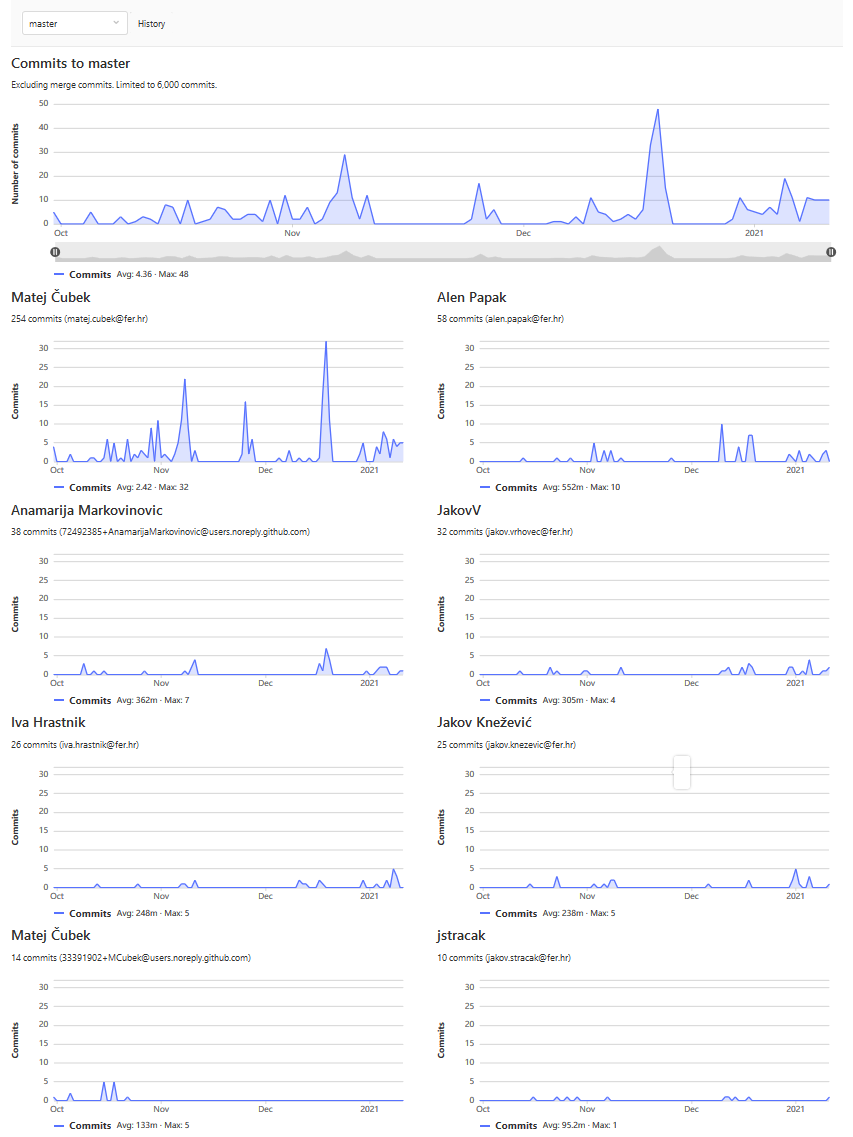
\includegraphics[scale=0.53]{slike/aktivnost} \\
			\caption{Dijagram promjena}
			\label{fig:dijagramPromjena}
		\end{figure}
		
	
